%% CPP 2027 submission skeleton — double-blind, sigplan format, 12 pp excl. refs/appendix.
%% Deadlines (AoE): abstract 2026-09-03, paper 2026-09-10.  Submit: https://cpp2027.hotcrp.com/
%% Build: latexmk -pdf main.tex
\documentclass[sigplan,screen,review,anonymous]{acmart}

%% TODO before camera-ready: drop `review,anonymous`, fill authors, rights form.
\setcopyright{none}
\acmConference[CPP '27]{Certified Programs and Proofs}{January 11--12, 2027}{Mexico City, Mexico}
\acmYear{2027}

\usepackage{listings}
\usepackage{amsmath}
\usepackage{tikz}
\usetikzlibrary{patterns,arrows.meta,positioning,decorations.pathreplacing,calc}

%% ---- Lean listings: minimal literate setup for the unicode we actually use ----
\lstdefinelanguage{lean}{
  keywords={theorem,def,structure,where,fun,by,exact,intro,obtain,refine,show,
            rcases,rw,omega,ring,calc,have,open,import,namespace,end,variable,abbrev},
  sensitive=true,
  comment=[l]{--},
  morecomment=[s]{/-}{-/},
  literate={≤}{{$\leq$}}1 {≥}{{$\geq$}}1 {∀}{{$\forall$}}1 {∃}{{$\exists$}}1
           {∈}{{$\in$}}1 {×}{{$\times$}}1 {⇒}{{$\Rightarrow$}}1 {→}{{$\to$}}1
           {ℕ}{{$\mathbb{N}$}}1 {ℂ}{{$\mathbb{C}$}}1 {≃}{{$\simeq$}}1
           {∧}{{$\wedge$}}1 {¬}{{$\neg$}}1 {∩}{{$\cap$}}1 {∪}{{$\cup$}}1
           {⟨}{{$\langle$}}1 {⟩}{{$\rangle$}}1 {≠}{{$\neq$}}1 {√}{{$\sqrt{}$}}1
           {Θ}{{$\Theta$}}1 {Ω}{{$\Omega$}}1 {μ}{{$\mu$}}1 {θ}{{$\theta$}}1 {ι}{{$\iota$}}1 {σ}{{$\sigma$}}1
           {□}{{$\square$}}1 {·}{{$\cdot$}}1 {↑}{{$\uparrow$}}1 {∉}{{$\notin$}}1,
}
\lstset{language=lean,basicstyle=\small\ttfamily,columns=fullflexible,
        keywordstyle=\bfseries,commentstyle=\itshape\color{gray},
        breaklines=true,frame=single,framerule=0.2pt,xleftmargin=1em}

\newcommand{\cc}{\mathrm{cc}}
\newcommand{\pw}{\mathrm{pw}}
\newcommand{\tw}{\mathrm{tw}}
\newcommand{\sys}{\textsc{FieldStemProof}}  % TODO: anonymize artifact name if identifying

\begin{document}

\title{How Far From Optimal Is Your Contraction Order?\\
       Machine-Checked Absolute Lower Bounds for Tensor-Network Contraction}
%% Alt titles (pick one):
%%   Certified Lower Bounds for Tensor-Network Contraction Ordering
%%   An Absolute Yardstick for Tensor-Network Contraction: Certified Cost Floors in Lean
%%   Below This Line No Contraction Order Exists: Certified TNCO Lower Bounds

\author{Anonymous Author(s)}
\affiliation{\institution{Anonymous Institution}\city{}\country{}}

\begin{abstract}
The cost of contracting a tensor network is governed by the contraction order, and finding an
optimal order (TNCO) is NP-hard. Practice therefore relies on heuristic search ---
hyper-optimized contraction trees, simulated annealing, community detection --- whose results
can only be judged \emph{relatively}: order $A$ beats order $B$, but how far either is from the
true optimum is unknown, because no trusted \emph{absolute} yardstick exists. We supply that
yardstick: machine-checked lower bounds on the cost of every \emph{sweep-style (stem)}
contraction order --- unconditionally --- extending to arbitrary contraction trees under a
single explicitly-stated published hypothesis ($\pw = \Theta(\tw)$ on lattices), formalized
in Lean~4 over Mathlib ($\sim$2{,}700 lines, no \texttt{sorry},
\textbf{zero custom axioms}). A trustworthy cost floor needs two independent ingredients, and
we certify both. First, a \emph{width} floor: a bramble is a combinatorial dual certificate for
pathwidth, and we prove the bramble bound self-contained via an elementary interval-Helly
argument --- the first pathwidth lower-bound theory in Lean. Second, width must genuinely
translate into cost: low-rank structure of intermediate tensors could undercut the width proxy
(this is exactly what decision-diagram methods exploit). Our \emph{Contraction Rigidity}
theorem closes this loophole structurally: any network \emph{capable} of full rank across a
cut has full rank for all tensor entries outside a proper subvariety --- no probability, and
the capability hypothesis reduces, via Kronecker routing, to a purely combinatorial cross-cut
matching. We instantiate the framework on a faithful model of the lattice family --- the
\emph{calibration} class, where the true optimum is independently known, so the tightness of
the yardstick is itself checkable --- with orders ranging over genuine path decompositions of
the circuit's spacetime lattice, widths derived, never postulated. At the Sycamore-53
benchmark scale the certificate is \emph{gap-free}: every stem order has width $\ge 54$ and
pays total cost $\ge 2^{54}$, our explicit sweep achieves width $\le 54$ --- the certified
floor \emph{meets} the found solution, i.e.\ the sweep carries a machine-checked proof of
optimality among stem orders --- and no low-rank factorization crosses the cut below inner
dimension $2^{53}$ generically.
%% TODO: final abstract pass; trim toward 200 words.
\end{abstract}

\begin{CCSXML}
<ccs2012>
<concept><concept_id>10003752.10003790.10011740</concept_id>
<concept_desc>Theory of computation~Type theory</concept_desc>
<concept_significance>500</concept_significance></concept>
<concept><concept_id>10003752.10003809.10010052</concept_id>
<concept_desc>Theory of computation~Quantum complexity theory</concept_desc>
<concept_significance>500</concept_significance></concept>
</ccs2012>
\end{CCSXML}
\ccsdesc[500]{Theory of computation~Type theory}
\ccsdesc[500]{Theory of computation~Quantum complexity theory}
\keywords{tensor networks, contraction ordering, lower bounds, optimality certificates,
Lean, Mathlib, pathwidth, brambles, Schwartz--Zippel, quantum circuit simulation}

\maketitle

%% ===================================================================
\section{Introduction}\label{sec:intro}

Contracting a tensor network is the workhorse of classical quantum-circuit simulation, and
its cost is governed almost entirely by one discrete choice: the \emph{contraction order}.
Choosing well is hard --- finding an optimal order is NP-hard on general
networks~\cite{markov2008simulating} --- so a decade of practice has produced a rich
ecosystem of heuristics: hyper-optimized contraction trees~\cite{gray2021hyper},
big-batch and index-slicing methods~\cite{pan2022solving}, stem-shaped orders for supremacy
circuits~\cite{huang2020classical}, multi-stem refinements~\cite{swtnc2025}, and
reuse-aware variants~\cite{kalachev2021recursive}. These tools are impressive, and they
share one methodological blind spot: \textbf{every quality judgment they support is
relative}. A new heuristic is validated by beating the previous one on a benchmark suite.
How far \emph{either} order is from the true optimum is unknown, because nothing trustworthy
bounds the optimum from below. ``State of the art'' means, literally, ``the best among the
orders we happened to find'' (Fig.~\ref{fig:yardstick}).

%% GEMINI-PROMPT (fallback if the TikZ below is replaced by an image):
%% "A clean schematic diagram, vector style, white background. A vertical axis labeled
%%  'contraction cost (log scale)'. On the upper part, three dots labeled 'order A', 'order B',
%%  'order C (best found)' connected by short curved arrows with labels 'beats' -- illustrating
%%  relative comparison. Below the dots, a large question-mark region labeled 'distance to
%%  optimum: unknown'. At the bottom, a thick horizontal line labeled 'certified floor
%%  (machine-checked theorem)' with the region below it hatched and labeled 'no contraction
%%  order exists here'. On the right margin, a bracket showing the gap between 'order C' and
%%  the floor labeled 'certified optimality gap'. Minimal colors: blue dots, red floor line,
%%  gray hatching."
\begin{figure}[t]
\centering
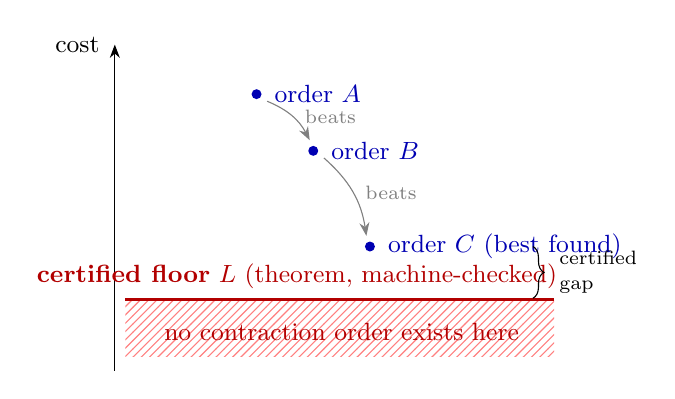
\begin{tikzpicture}[scale=0.9, font=\small]
  % axis
  \draw[-{Stealth}] (0,0) -- (0,4.6) node[left=2pt] {cost};
  % hatched forbidden region
  \fill[pattern=north east lines, pattern color=red!50] (0.15,0.2) rectangle (6.2,1.0);
  \draw[red!70!black, very thick] (0.15,1.0) -- (6.2,1.0)
    node[pos=0.4, above] {\textbf{certified floor} $L$ (theorem, machine-checked)};
  \node[red!70!black] at (3.2,0.55) {no contraction order exists here};
  % found orders
  \fill[blue!70!black] (2.0,3.9) circle (2pt) node[right=3pt] {order $A$};
  \fill[blue!70!black] (2.8,3.1) circle (2pt) node[right=3pt] {order $B$};
  \fill[blue!70!black] (3.6,1.75) circle (2pt) node[right=3pt] {order $C$ (best found)};
  \draw[-{Stealth}, gray] (2.15,3.8) to[bend left=20]
    node[midway, right=1pt] {\scriptsize beats} (2.75,3.25);
  \draw[-{Stealth}, gray] (2.95,3.0) to[bend left=20]
    node[midway, right=1pt] {\scriptsize beats} (3.55,1.9);
  % gap brace
  \draw[decorate, decoration={brace, amplitude=4pt}] (5.9,1.75) -- (5.9,1.02)
    node[midway, right=6pt, align=left] {\scriptsize certified\\[-2pt]\scriptsize gap};
\end{tikzpicture}
\caption{Relative vs.\ absolute evaluation of contraction orders. Heuristics can rank found
orders against each other (top), but only a certified lower bound (bottom) turns the best
found order into a solution with a provable optimality gap. On our calibration instance the
floor \emph{meets} the found sweep: the gap is zero.}
\label{fig:yardstick}
\end{figure}

What is missing is an \emph{absolute yardstick}: a trusted bound $L$ together with a proof
that \emph{no} contraction order costs less than $L$. With such a floor, any found order $S$
acquires a certificate --- $\mathrm{cost}(S)/L$ bounds its optimality gap --- exactly as an
LP dual bound certifies a branch-and-bound incumbent, or an UNSAT certificate closes a SAT
search. Nothing of this kind has existed for TNCO.

Why not? Because a \emph{trustworthy} cost floor must survive three independent attacks, and
each attack has historically been fatal (Fig.~\ref{fig:floors}). First, the graph-theoretic
width bound underlying the floor may simply be wrong: lower-bound proofs in width theory are
subtle, and an unverified bound certifies nothing. Second, width may fail to translate into
cost: width counts indices of the largest intermediate tensor, and if that tensor has
low-rank structure, a cleverer representation pays less --- decision-diagram simulators
demonstrably break the width proxy on structured instances~\cite{dd2025treewidth}. Third,
the translation must hold for the \emph{instances at hand}, not just in the worst case:
random shallow circuits are classically easy despite large width~\cite{napp2022efficient}.
Our response to all three is the same: make every link a machine-checked theorem, and split
the labor so that \emph{search may be heuristic but trust never is} --- finding a good
bramble (the dual certificate below) is a search problem; \emph{validating} one is a
verified theorem.

%% GEMINI-PROMPT (fallback):
%% "A clean vertical stack of three rounded rectangles, vector style, like an architecture
%%  diagram. Top box: 'Width floor -- bramble = dual certificate (interval Helly)', with a
%%  crossed-out attack arrow labeled 'unverified graph bound'. Middle box: 'Cost floor --
%%  cost(o) = sum of 2^|bag|', attack arrow crossed out labeled 'width is only a proxy'.
%%  Bottom box: 'Compression floor -- Contraction Rigidity: generically no low-rank
%%  factorization', attack arrow crossed out labeled 'decision-diagram / MPS escape'.
%%  Right side annotations in monospace: theorem names grid_pathwidth_exact,
%%  gridModel_cost_floor, no_compression. Muted professional colors."
\begin{figure}[t]
\centering
\resizebox{\columnwidth}{!}{%
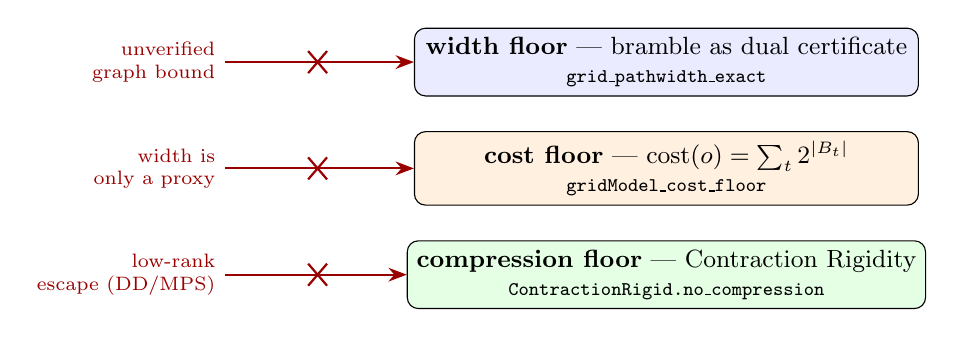
\begin{tikzpicture}[font=\small,
  atk/.style={-{Stealth}, thick, red!60!black}]
  \node[draw, rounded corners, fill=blue!8, minimum width=6.4cm, align=center] (w) at (0,2.7)
    {\textbf{width floor} --- bramble as dual certificate\\[-1pt]
     {\scriptsize\ttfamily grid\_pathwidth\_exact}};
  \node[draw, rounded corners, fill=orange!12, minimum width=6.4cm, align=center] (c) at (0,1.35)
    {\textbf{cost floor} --- $\mathrm{cost}(o)=\sum_t 2^{|B_t|}$\\[-1pt]
     {\scriptsize\ttfamily gridModel\_cost\_floor}};
  \node[draw, rounded corners, fill=green!10, minimum width=6.4cm, align=center] (r) at (0,0)
    {\textbf{compression floor} --- Contraction Rigidity\\[-1pt]
     {\scriptsize\ttfamily ContractionRigid.no\_compression}};
  \draw[atk] (-5.6,2.7) node[left, align=right, font=\scriptsize]
    {unverified\\graph bound} -- (w.west);
  \draw[atk] (-5.6,1.35) node[left, align=right, font=\scriptsize]
    {width is\\only a proxy} -- (c.west);
  \draw[atk] (-5.6,0) node[left, align=right, font=\scriptsize]
    {low-rank\\escape (DD/MPS)} -- (r.west);
  \foreach \y in {2.7,1.35,0} {\draw[red!60!black, thick]
    (-4.55,\y-0.14) -- (-4.31,\y+0.14) (-4.55,\y+0.14) -- (-4.31,\y-0.14);}
\end{tikzpicture}}
\caption{A trustworthy cost floor blocks three attacks with three certified layers; each
layer is a named Lean theorem with standard axioms only.}
\label{fig:floors}
\end{figure}

This paper delivers that yardstick, formalized in Lean~4 over
Mathlib~\cite{moura2021lean,mathlib2020}: $\sim$2{,}700 lines, 17 modules, no
\texttt{sorry}, zero custom axioms --- \texttt{\#print axioms} of every theorem below
reports only \texttt{propext}, \texttt{Classical.choice}, \texttt{Quot.sound}. The
unconditional floors quantify over all \emph{sweep-style (stem)} orders --- the class that
state-vector-like simulators and stem-shaped supremacy strategies actually
populate~\cite{huang2020classical} --- and extend to arbitrary contraction trees under a
single explicitly-stated published hypothesis ($\pw = \Theta(\tw)$ on lattices), carried in
theorem statements rather than assumed globally.

\paragraph{Contributions.}
\begin{itemize}
  \item \textbf{An absolute yardstick for TNCO (\S\ref{sec:framework},\S\ref{sec:model}).}
    A formal cost/width model in which ``no contraction order beats bound $L$'' is a
    theorem quantified over a \emph{genuine} order space --- real path decompositions of
    the network graph, widths derived, never postulated --- with an explicit cost object:
    \lstinline|orderCost| sums the materialized boundary tensors, and the certified floor
    is a \emph{cost} statement (\lstinline|gridModel_cost_floor|:
    $2^{N+1} \le \mathrm{cost}(o)$ for every order $o$ of the $N \times N$ lattice), not
    merely a width statement.
  \item \textbf{Bramble certificates in Lean (\S\ref{sec:bramble}).} Brambles are
    combinatorial \emph{dual certificates} for width, playing the role LP duality plays for
    branch-and-bound floors: however a bramble is found --- by hand, by heuristic search ---
    the checked theorem turns it into an absolute floor. Stem (sweep) orders are exactly
    path decompositions, whose dual argument needs only \emph{interval} Helly ---
    elementary, unlike the subtree Helly that treewidth needs and Mathlib lacks. We prove
    the bound for genuine \emph{touching} brambles (blocks intersecting \emph{or} adjacent)
    and instantiate two: the elementary crosses (order $\Theta(k)$) and the augmented
    Seymour--Thomas-style bramble (\S\ref{sec:exact}), whose order $k+2$ pins the grid
    floor \emph{exactly}. The first pathwidth lower-bound theory in Lean/Mathlib.
  \item \textbf{Contraction Rigidity: width $\Rightarrow$ cost, generically
    (\S\ref{sec:rigidity}).} A width floor is only a cost floor if intermediate tensors do
    not collapse in rank. We close this loophole structurally: \lstinline|BulkEntangling|
    $\Rightarrow$ \lstinline|ContractionRigid| --- one full-rank configuration upgrades to
    full rank outside a proper subvariety (Schwartz--Zippel, no probability); the
    hypothesis reduces via Kronecker routing to a combinatorial cross-cut matching.
    The payoff is a formal \emph{no-compression theorem}
    (\lstinline|ContractionRigid.no_compression|): generically, the cut flattening admits
    no factorization with inner dimension below $2^k$ --- no MPS-style bond, no
    rank-revealing compression undercuts the floor (the decision-diagram loophole),
    except on a measure-zero set of instances.
  \item \textbf{A gap-free certified benchmark instance (\S\ref{sec:endtoend}).} At the
    Sycamore-53 scale, one machine-checked theorem pins the optimum exactly:
    $\cc = 54$ (\lstinline|sycamore53_cc_exact|), every stem order pays total cost
    $\ge 2^{54}$ (\lstinline|sycamore53_cost_floor|), the cut is fenced against
    factorizations of inner dimension $< 2^{53}$ for generic gate values
    (\lstinline|sycamore53_bond_floor|), and the explicit sweep attains the floor --- a
    found solution carrying a machine-checked \emph{optimality proof}, with
    \texttt{\#print axioms} reporting standard axioms only.
  \item \textbf{Geometric routing (\S\ref{sec:routing}).} The matching hypothesis is
    realized on real hardware graphs: the $b\cdot d$ depth cap is a gate-counting theorem,
    and bond reachability is an explicit lightcone walk on 1D chains and 2D chips.
\end{itemize}

%% ===================================================================
\section{Background}\label{sec:background}

\subsection{Tensor networks, orders, and width}
A quantum circuit compiles into a tensor network: one tensor per gate, one shared index per
wire. Simulating the circuit means contracting the network to a scalar, and a
\emph{contraction order} schedules the pairwise merges. The cost of an order is dominated by
its widest intermediate tensor: an intermediate with $w$ open indices holds $2^w$ entries.
Markov and Shi~\cite{markov2008simulating} identified the optimal width over all orders with
the treewidth of the network's line graph, which pins the complexity of the
\emph{contraction paradigm} (including index slicing, which trades memory for time but not
total work). Two caveats scope everything that follows. The paradigm bound is not an
unconditional hardness claim: representations exploiting \emph{value} structure ---
stabilizer states, decision diagrams~\cite{dd2025treewidth} --- can beat width on structured
instances, and shallow random 2D circuits are classically easy outright%
~\cite{napp2022efficient}. Our floors therefore live in the contraction paradigm, and
\S\ref{sec:rigidity} shows that for \emph{generic} tensor entries even the value-structure
escape is closed. Second, NP-hardness of TNCO is a statement about general networks; on
planar grids the width is textbook-known --- which is precisely what will qualify the
lattice family as a \emph{calibration} class in \S\ref{sec:endtoend}.

\subsection{Stem orders are path decompositions}
The orders that dominate practice on supremacy-style circuits are
\emph{stems}~\cite{huang2020classical}: a single growing tensor absorbs the network one
piece at a time, exactly like a state vector swept through a circuit. In tree language the
contraction tree is a caterpillar --- a spine with leaves. The combinatorial identity at
the heart of this paper (Fig.~\ref{fig:stemsweep}) is that \textbf{a stem order is the same
data as a path decomposition} of the network graph: the $t$-th bag $B_t$ is the boundary of
the absorbed region after $t$ steps, the width of the order is the largest bag, and the
optimal stem width is the pathwidth. This identity is what makes certified floors for stem
orders tractable today: pathwidth lower bounds rest on \emph{interval} Helly
(\S\ref{sec:bramble}), a one-dimensional argument, where treewidth would need the subtree
Helly property that Mathlib does not yet have.

%% GEMINI-PROMPT (fallback):
%% "Two-panel scientific diagram, vector style. Left panel: a 5x5 grid of small circles
%%  connected by lines (a lattice tensor network); a bold dashed vertical-ish frontier line
%%  separates a shaded 'absorbed' region on the left from the rest; the circles on the
%%  frontier are highlighted orange and labeled 'bag B_t = boundary'. An arrow labeled
%%  'sweep' points rightward. Right panel: a caterpillar tree: a horizontal bold path of 6
%%  nodes (the spine), each spine node with one or two small leaf nodes hanging below;
%%  caption inside: 'stem contraction tree'. Between panels a double arrow labeled 'same
%%  data'. Minimal colors: gray network, orange bag, blue spine."
\begin{figure}[t]
\centering
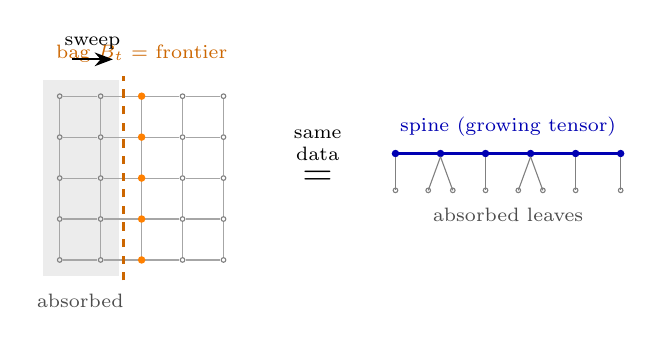
\begin{tikzpicture}[scale=0.52, font=\scriptsize]
  % ---- left: grid with sweep frontier ----
  \begin{scope}
    % absorbed region shading (columns 0-1, plus column 2 partially)
    \fill[gray!15] (-0.4,-0.4) rectangle (1.45,4.4);
    \foreach \x in {0,...,4} \foreach \y in {0,...,4} {
      \draw[gray] (\x,\y) circle (1.6pt);
      \ifnum\x<4 \draw[gray!70] (\x+0.08,\y) -- (\x+0.92,\y); \fi
      \ifnum\y<4 \draw[gray!70] (\x,\y+0.08) -- (\x,\y+0.92); \fi
    }
    % frontier bag: column 2 vertices highlighted
    \foreach \y in {0,...,4} \fill[orange] (2,\y) circle (2.6pt);
    \draw[very thick, dashed, orange!80!black] (1.55,-0.5) -- (1.55,4.5);
    \node[orange!80!black] at (2.0,5.05) {bag $B_t$ = frontier};
    \node[gray!60!black] at (0.5,-1.0) {absorbed};
    \draw[-{Stealth}, thick] (0.3,4.9) -- (1.3,4.9) node[midway, above] {sweep};
  \end{scope}
  % ---- middle: equivalence ----
  \node at (6.3,2) {\Large$\;=\;$};
  \node[align=center] at (6.3,2.8) {same\\data};
  % ---- right: caterpillar tree ----
  \begin{scope}[shift={(8.2,0)}]
    \foreach \i in {0,...,5} \fill[blue!70!black] (\i*1.1,2.6) circle (2.6pt);
    \foreach \i in {0,...,4} \draw[blue!70!black, very thick]
      (\i*1.1+0.07,2.6) -- (\i*1.1+1.03,2.6);
    \foreach \i/\n in {0/1,1/2,2/1,3/2,4/1,5/1} {
      \ifnum\n=1
        \draw[gray] (\i*1.1,2.52) -- (\i*1.1,1.7); \draw[gray] (\i*1.1,1.7) circle (1.6pt);
      \else
        \draw[gray] (\i*1.1,2.52) -- (\i*1.1-0.3,1.7); \draw[gray] (\i*1.1-0.3,1.7) circle (1.6pt);
        \draw[gray] (\i*1.1,2.52) -- (\i*1.1+0.3,1.7); \draw[gray] (\i*1.1+0.3,1.7) circle (1.6pt);
      \fi
    }
    \node[blue!70!black] at (2.75,3.25) {spine (growing tensor)};
    \node[gray!60!black] at (2.75,1.1) {absorbed leaves};
  \end{scope}
\end{tikzpicture}
\caption{A stem (caterpillar) contraction order \emph{is} a path decomposition: the spine's
$t$-th intermediate tensor has exactly the frontier bag $B_t$ as its open indices. Width of
the order $=$ largest bag; optimal stem width $=$ pathwidth.}
\label{fig:stemsweep}
\end{figure}

\subsection{The sweep cut and the benchmark scale}
For an $n$-qubit depth-$d$ lattice circuit the two canonical sweeps give cut sizes $n$
(time sweep) and $\lfloor\sqrt{n}\rfloor\cdot d$ (space sweep), so the achievable width
scale is $\mathrm{sweepCut}(n,d)=\min(n,\lfloor\sqrt{n}\rfloor d)$; at the Sycamore-53
parameters $(n,d)=(53,20)$ this is $53$, and the folklore cost estimate
$4\cdot 2^{53}\cdot 150 \approx 10^{18}$ is pure arithmetic that our development also
certifies (\lstinline|CorollaryD|). Throughout, ``Sycamore-53 scale'' refers to these
parameters; the lattice we instantiate is the deep-regime spacetime grid of a wire chain
(\S\ref{sec:endtoend} discusses fidelity scope).

\subsection{Lean 4 and Mathlib}
The development is built on Lean~4 and Mathlib (both pinned at v4.30.0), using
\lstinline|SimpleGraph| box products for lattices, \lstinline|Finset| combinatorics for
brambles and transversals, and \lstinline|MvPolynomial| with matrix determinants for the
genericity engine. The auditing interface is \texttt{\#print axioms}: every theorem cited in
this paper reports \texttt{[propext, Classical.choice, Quot.sound]} --- no custom axiom
exists anywhere in the library, and the one literature input we rely on
($\pw=\Theta(\tw)$ on lattices) appears as an explicit hypothesis \emph{inside} theorem
statements, never as an ambient assumption.

%% ===================================================================
\section{The Formal Framework}\label{sec:framework}
%% Defs.lean: QTensor, cutEquiv, flatten, squareFlatten, tensorOfMatrix, bellWitness.
%% Key design: flattening across a cut as the *only* interface between graph combinatorics
%% and linear algebra; eval commutes with flatten (flatten_map) transports genericity.
\begin{lstlisting}
abbrev QTensor (I R : Type*) := (I → Fin 2) → R

def flatten (T : QTensor I R) :
    Matrix ({i // p i} → Fin 2) ({i // ¬ p i} → Fin 2) R :=
  Matrix.of fun a b => T ((cutEquiv p).symm (a, b))
\end{lstlisting}
%% CircuitGraph abstraction (Order, width, IsStem, cc = sInf, pw = sInf over stems);
%% proved skeleton: cc_le_pw, exists_stem_pw, optimal_stem_within_const.

%% ===================================================================
\section{Contraction Rigidity}\label{sec:rigidity}
%% LemmaB.lean: generic_nonsingular (the engine). Rigidity.lean: BulkEntangling,
%% ContractionRigid, contraction_rigidity. Matching.lean: Kronecker routing
%% det_bondProd_ne_zero; matching_contractionRigid with explicit matching data.
%% Gates.lean + Worstcase.lean: the hypothesis is non-vacuous for real gate sets
%% (X..fSim all nonsingular; iSWAP/CNOT/fSim realize full Schmidt rank).
\begin{lstlisting}
theorem contraction_rigidity
    (e : ({i // p i} → Fin 2) ≃ ({i // ¬ p i} → Fin 2))
    {T : QTensor I (MvPolynomial ι K)}
    (h : BulkEntangling p e T) : ContractionRigid p e T
\end{lstlisting}

%% GEMINI-PROMPT (fallback):
%% "Schematic diagram, vector style: two columns of 4 qubits each (circles labeled L1..L4
%%  and R1..R4), separated by a vertical dashed line labeled 'cut'. Each pair (Lj, Rj) is
%%  connected by a bold edge labeled 'B_j, det != 0' (a two-qubit entangling bond). Below,
%%  an equation-style annotation: 'flattening = B_1 (x) B_2 (x) B_3 (x) B_4, full rank 2^4'.
%%  A side note: 'one full-rank configuration => full rank for all generic parameters
%%  (Schwartz-Zippel)'. Minimal colors: blue bonds, gray qubits."
\begin{figure}[t]
\centering
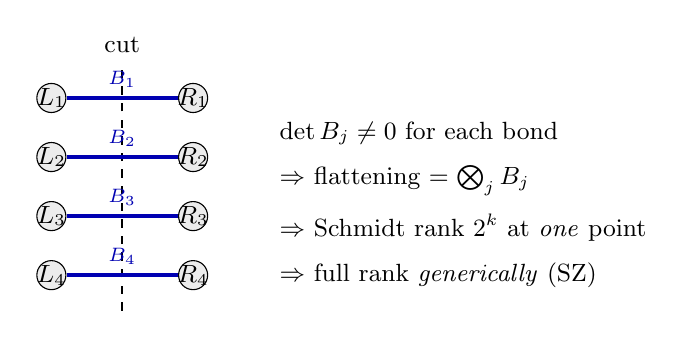
\begin{tikzpicture}[scale=0.75, font=\small]
  \draw[dashed, thick] (2.1,-0.6) -- (2.1,3.6) node[above] {cut};
  \foreach \y/\j in {0/4,1/3,2/2,3/1} {
    \draw[fill=gray!15] (0.9,\y) circle (7pt) node {$L_{\j}$};
    \draw[fill=gray!15] (3.3,\y) circle (7pt) node {$R_{\j}$};
    \draw[blue!70!black, very thick] (1.16,\y) -- (3.04,\y)
      node[midway, above] {\scriptsize $B_{\j}$};
  }
  \node[align=left, anchor=west] at (4.6,2.4)
    {$\det B_j \neq 0$ for each bond};
  \node[align=left, anchor=west] at (4.6,1.6)
    {$\Rightarrow$ flattening $=\bigotimes_j B_j$};
  \node[align=left, anchor=west] at (4.6,0.8)
    {$\Rightarrow$ Schmidt rank $2^{k}$ at \emph{one} point};
  \node[align=left, anchor=west] at (4.6,0.0)
    {$\Rightarrow$ full rank \emph{generically} (SZ)};
\end{tikzpicture}
\caption{Kronecker routing reduces the rigidity hypothesis to combinatorics: a cross-cut
perfect matching with nonsingular bonds makes the cut flattening a Kronecker product, hence
full rank at one gate configuration --- and Schwartz--Zippel upgrades one point to all
generic parameters. No probability enters.}
\label{fig:matching}
\end{figure}
%% Punchline: the average-case question is *structural*, not probabilistic; the
%% probability-zero corollary (C.3) is future work but follows from measure-zero varieties.

%% ===================================================================
\section{Stem Width via Interval Helly}\label{sec:bramble}
%% Bramble.lean: interval_helly -> some_bag_hits_all -> order_le_maxBag(')
%% -> pathwidth_ge_order_of_connected / pathwidth_ge_order_of_touching.
%% Design insight: pathwidth needs only 1D Helly. Two bound forms:
%%  - intersecting blocks (elementary crosses: k <= 2·order, projection counting);
%%  - touching blocks (intersect OR adjacent; shared bag comes from the edge-cover
%%    axiom) -- the genuine bramble condition, needed for augmented brambles.
%% GridConn.lean: crosses are connected in the true grid (box-product walk embeddings);
%% grid_pathwidth_lower_unconditional: k <= 2·maxBag, no hypotheses left.
%% GEMINI-PROMPT (fallback):
%% "Diagram, vector style: a horizontal row of 8 rectangles labeled B1..B8 (bags of a path
%%  decomposition). Above them, three horizontal colored bars (blue, orange, green) at
%%  different heights, each spanning a contiguous range of bags (blue spans B2-B6, orange
%%  B4-B8, green B1-B5). All three bars overlap around B4-B5. A vertical dashed line drops
%%  through bag B5, labeled 'common bag: meets every block (interval Helly)'. Caption
%%  concept: connected blocks occupy bag-intervals; pairwise touching makes intervals
%%  pairwise overlap; Helly for intervals yields one bag hitting all blocks."
\begin{figure}[t]
\centering
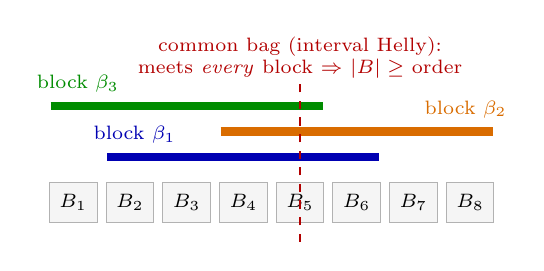
\begin{tikzpicture}[scale=0.72, font=\scriptsize]
  % bags
  \foreach \i in {1,...,8} {
    \draw[gray!60, fill=gray!8] (\i-0.42,0) rectangle (\i+0.42,0.7);
    \node at (\i,0.35) {$B_{\i}$};
  }
  % interval bars
  \draw[blue!70!black,   line width=3pt] (1.6,1.15) -- (6.4,1.15)
    node[pos=0.1, above] {block $\beta_1$};
  \draw[orange!85!black, line width=3pt] (3.6,1.6)  -- (8.4,1.6)
    node[pos=0.9, above] {block $\beta_2$};
  \draw[green!55!black,  line width=3pt] (0.6,2.05) -- (5.4,2.05)
    node[pos=0.1, above] {block $\beta_3$};
  % common bag
  \draw[dashed, thick, red!70!black] (5,-0.35) -- (5,2.5);
  \node[red!70!black, align=center] at (5,2.9)
    {common bag (interval Helly):\\meets \emph{every} block $\Rightarrow$ $|B|\ge$ order};
\end{tikzpicture}
\caption{The pathwidth dual argument. A connected block meets the bags of a path
decomposition along a contiguous \emph{interval} of indices; pairwise-touching blocks give
pairwise-overlapping intervals; interval Helly (the maximal left endpoint) produces one bag
meeting all blocks, so the largest bag is at least the bramble's transversal order. Only
one-dimensional Helly is needed --- this is why stem-order floors are formalizable today.}
\label{fig:helly}
\end{figure}

\begin{lstlisting}
theorem grid_pathwidth_lower_unconditional (k : ℕ) (hk : 0 < k)
    (L : LinearBags (Fin k × Fin k)) (hlen : 0 < L.len)
    (hvint : ...) (hedge : ...) (hcov : ...) :
    k ≤ 2 * L.maxBag hlen
\end{lstlisting}

%% ===================================================================
\section{The Exact Floor: an Augmented Bramble}\label{sec:exact}
%% GridExact.lean. For a yardstick, the constant matters: Θ(k) with slack factor 2 is a
%% weak certificate; the augmented (Seymour--Thomas style) bramble closes the gap.
%% - Blocks: k² subgrid crosses ⊕ last row ⊕ last column minus corner; boundary blocks
%%   are disjoint from the crosses and touch only through edges -> touching bound.
%% - Monotone chain walks with support bounds (subgrid arms must not overshoot).
%% - Transversal counting (the classical "miss a row and a column" argument, by
%%   projections): order ≥ k + 2.
%% - Punchline: floor k+2 meets the sliding-window sweep exactly -- the grid stem
%%   optimum is PINNED, and the sweep is provably optimal among stem orders.
%% GEMINI-PROMPT (fallback):
%% "Diagram of a 6x6 grid of circles (a (k+1)x(k+1) lattice with k=5). The top-left 5x5
%%  subgrid is tinted light blue. One sample 'cross' inside the subgrid is highlighted:
%%  all circles of subgrid-row i and subgrid-column j in saturated blue, meeting at (i,j).
%%  The entire last row is red. The last column except its bottom-right corner is green.
%%  Two short zigzag marks highlight edges where blue touches red and blue touches green
%%  (adjacent but disjoint blocks). Side annotation: 'transversal must contain: 1 red +
%%  1 green + (k) blue-region vertices, else some row i0 AND column j0 are both missed and
%%  cross (i0,j0) is unhit => order >= k+2'."
\begin{figure}[t]
\centering
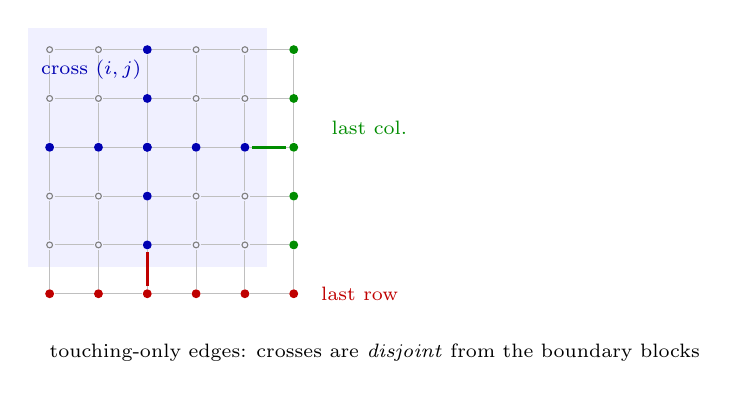
\begin{tikzpicture}[scale=0.62, font=\scriptsize]
  \def\k{5}
  % subgrid tint
  \fill[blue!6] (-0.45,0.55) rectangle (4.45,5.45);
  % lattice edges
  \foreach \x in {0,...,5} \foreach \y in {0,...,5} {
    \ifnum\x<5 \draw[gray!50] (\x+0.1,\y) -- (\x+0.9,\y); \fi
    \ifnum\y<5 \draw[gray!50] (\x,\y+0.1) -- (\x,\y+0.9); \fi
  }
  % base vertices
  \foreach \x in {0,...,5} \foreach \y in {0,...,5} \draw[gray] (\x,\y) circle (1.7pt);
  % sample cross: subgrid row y=3 and column x=2 (rows 1..5 are subgrid here; last row y=0)
  \foreach \x in {0,...,4} \fill[blue!70!black] (\x,3) circle (2.6pt);
  \foreach \y in {1,...,5} \fill[blue!70!black] (2,\y) circle (2.6pt);
  \node[blue!70!black] at (0.85,4.6) {cross $(i,j)$};
  % last row (y=0) red
  \foreach \x in {0,...,5} \fill[red!75!black] (\x,0) circle (2.6pt);
  \node[red!75!black] at (6.35,0) {last row};
  % last column (x=5) minus corner green
  \foreach \y in {1,...,5} \fill[green!55!black] (5,\y) circle (2.6pt);
  \node[green!55!black] at (6.55,3.4) {last col.};
  % touching marks
  \draw[very thick, red!75!black]   (2,0.15) -- (2,0.85);
  \draw[very thick, green!55!black] (4.15,3) -- (4.85,3);
  \node[align=left, anchor=west] at (-0.2,-1.2)
    {touching-only edges: crosses are \emph{disjoint} from the boundary blocks};
\end{tikzpicture}
\caption{The augmented bramble on the $(k{+}1)\times(k{+}1)$ grid: $k^2$ subgrid crosses
(blue), the last row (red), and the last column minus the corner (green). Boundary blocks
touch the crosses only through edges, which the touching-bramble bound
(\lstinline|pathwidth_ge_order_of_touching|) handles via the edge-cover axiom. Counting: a
transversal needs one red, one green, and $k$ subgrid vertices --- otherwise some row $i_0$
\emph{and} some column $j_0$ are missed and cross $(i_0,j_0)$ is unhit --- so the order is
$\ge k+2$, meeting the sweep exactly.}
\label{fig:augmented}
\end{figure}

\begin{lstlisting}
theorem grid_pathwidth_exact (k : ℕ) (hk : 0 < k)
    (L : LinearBags (Fin (k+1) × Fin (k+1))) (hlen : 0 < L.len)
    (hvint : ...) (hedge : ...) (hcov : ...) :
    k + 2 ≤ L.maxBag hlen
\end{lstlisting}

%% ===================================================================
\section{A Faithful Circuit Model}\label{sec:model}
%% GridModel.lean. The degeneracy story is worth telling honestly:
%% v1 model had Order := Unit, width := const 53 -- the stem clause was near-vacuous.
%% v2: Order = { L : LinearBags // IsPathDecomp k L }, width = actual largest bag.
%% Lower: augmented-bramble theorem (exact). Upper: sliding-window sweep (bag t =
%% positions [t, t+k]), card <= k+1 by injectivity of column-major position into an Icc
%% window. cc = N+1 exactly (gridModel_cc_eq); optimum attained (Nat.sInf_mem);
%% cost object: orderCost = Σ 2^|bag|; cost floor 2^{N+1} (gridModel_cost_floor);
%% LatticePathwidthBound holds with C = 1 by construction (order space = stems).
%% GEMINI-PROMPT (fallback):
%% "Diagram: a 5x5 grid of circles with small numbers 0..24 written column-major (down each
%%  column then next column). Circles with numbers < 8 are filled gray ('absorbed'). Circles
%%  numbered 8..13 have bold orange rings ('window = bag, k+1 = 6 vertices'). Circles > 13
%%  are white ('future'). A legend below. Concept: sweeping vertices in column-major order;
%%  the bag at step t is the sliding window of positions [t, t+k]."
\begin{figure}[t]
\centering
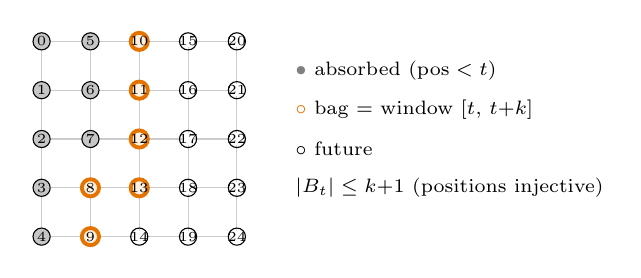
\begin{tikzpicture}[scale=0.62, font=\tiny]
  \foreach \x in {0,...,4} \foreach \y in {0,...,4} {
    \ifnum\x<4 \draw[gray!40] (\x+0.12,4-\y) -- (\x+0.88,4-\y); \fi
    \ifnum\y<4 \draw[gray!40] (\x,4-\y-0.88) -- (\x,4-\y-0.12); \fi
  }
  \foreach \x in {0,...,4} \foreach \y in {0,...,4} {
    \pgfmathtruncatemacro{\p}{\x*5+\y}
    \ifnum\p<8
      \draw[fill=gray!45] (\x,4-\y) circle (5pt); \node at (\x,4-\y) {\p};
    \else\ifnum\p<14
      \draw[line width=1.4pt, orange!90!black, fill=orange!12] (\x,4-\y) circle (5pt);
      \node at (\x,4-\y) {\p};
    \else
      \draw (\x,4-\y) circle (5pt); \node at (\x,4-\y) {\p};
    \fi\fi
  }
  \node[align=left, anchor=west, font=\scriptsize] at (5.0,3.4)
    {\textcolor{gray}{$\bullet$} absorbed ($\mathrm{pos}<t$)};
  \node[align=left, anchor=west, font=\scriptsize] at (5.0,2.6)
    {\textcolor{orange!90!black}{$\circ$} bag $=$ window $[t,\,t{+}k]$};
  \node[align=left, anchor=west, font=\scriptsize] at (5.0,1.8)
    {$\circ$ future};
  \node[align=left, anchor=west, font=\scriptsize] at (5.0,1.0)
    {$|B_t| \le k{+}1$ (positions injective)};
\end{tikzpicture}
\caption{The sliding-window sweep (\texttt{sweepBags}, shown at $t=8$ on the $5\times5$
grid): vertices are absorbed in column-major position order; the bag at step $t$ is the
window of positions $[t, t+k]$ --- the live frontier plus the vertex being absorbed. Each
window holds at most $k+1$ vertices, realizing the textbook grid pathwidth and meeting the
floor of Fig.~\ref{fig:augmented}.}
\label{fig:window}
\end{figure}

\begin{lstlisting}
def gridModel (k : ℕ) : CircuitGraph where
  Order  := {L : LinearBags (Fin k × Fin k) // IsPathDecomp k L}
  width  := fun o => bagsWidth o.1
  IsStem := fun _ => True
  ...
\end{lstlisting}

%% ===================================================================
\section{Case Study: a Gap-Free Certified Benchmark Instance}\label{sec:endtoend}
%% Sycamore-53 as the calibration instance: the lattice family is where the true optimum
%% is independently known, so the yardstick's tightness is itself checkable -- and it reads
%% exactly right (floor = sweep = 54).
%% CorollaryD.lean (pure arithmetic): sweepCut 53 20 = 53; 10^18 <= 4·2^53·150 < 10^19.
%% Sycamore.lean: the four-conjunct theorem; #print axioms = standard only.
%% Read the theorem as a certificate: (i) exact floor -- cc = 54, no stem order below 54;
%% (ii) optimality proof -- the sweep is a *found solution* attaining the floor;
%% (iii) cost semantics -- every order pays ≥ 2^54; (iv) rigidity -- generic values leave
%% no low-rank escape below inner dimension 2^53.
\begin{lstlisting}
theorem sycamore53_lower_bound :
    CorollaryD.sweepCut 53 20 = 53 ∧
    ((10:ℕ)^18 ≤ CorollaryD.stemCost 53 20 150 ∧
      CorollaryD.stemCost 53 20 150 < (10:ℕ)^19) ∧
    (sycamore53.cc = 54 ∧
      (∃ o, sycamore53.IsStem o ∧
        sycamore53.width o = sycamore53.cc) ∧
      (∀ o : sycamore53.Order,
        2 ^ 54 ≤ GridModel.orderCost o)) ∧
    (∃ e T, ContractionRigid leftBlock e T)
\end{lstlisting}

%% ===================================================================
\section{Geometric Routing: Brickwork and Lightcones}\label{sec:routing}
%% Brickwork.lean: Schedule (d layers, <= b straddling gates each); routed_card_le
%% proves the b·d cap (card_biUnion_le_card_mul); min(n, b·d) achieved; keystone:
%% deep_brickwork_contractionRigid at size sweepCut.
%% Causal.lean: bonds are chip qubit pairs within the depth-d lightcone; chain_reach
%% (1D, exact-length walks); grid_bond_causal (2D chip via boxProd walk lifting);
%% K·min(m,d) = min(n/2, √n·d) on square chips.

%% ===================================================================
\section{Related Work}\label{sec:related}
%% Organize around the yardstick framing:
%% - TNCO heuristics (all relative): Gray--Kourtis hyper-opt; Pan--Zhang big-batch;
%%   Huang et al. stems; SW-TNC multi-stem; Kalachev et al. reuse. None certify a gap.
%% - Width machinery: Markov--Shi (cc = tw); Boixo et al. (grid tw estimates, QuickBB
%%   heuristic -- again relative); treewidth exact solvers (small instances, unverified).
%%   Scope honestly: TNCO hardness is about general networks; on grids the width is
%%   textbook-known -- which is precisely what qualifies the lattice family as the
%%   calibration class for the yardstick.
%% - The loopholes we close: Napp et al. (shallow-2D simulable phase -> regime hypothesis);
%%   decision diagrams break the width proxy on structured values -> rigidity fences
%%   generic values.
%% - Formalization: Doczkal--Pous (Coq graph theory, treewidth-two); TNLean / multi-agent
%%   autoformalization of MPS (different scope: no contraction complexity); no prior Lean
%%   pathwidth/treewidth or TN-contraction development.
%% - Certified-bound analogues in other fields: verified LP/SAT certificates, proof-carrying
%%   branch-and-bound floors -- brambles play the dual-certificate role here, and the
%%   checker-vs-search division (heuristic bramble hunting, verified certificate) mirrors
%%   verified SAT/LP checking.

\section{Limitations and Future Work}\label{sec:limits}
%% Honest certificate-scope list, mirrors docs §4:
%% 1. The unconditional floor quantifies over stem (linear) orders; extending to all tree
%%    orders is the pw = Θ(tw) literature input, carried as an explicit hypothesis in the
%%    statements (formalizing subtree Helly + tree decompositions removes it; journal
%%    version). State plainly: today's certificate says "no sweep-style order beats 54";
%%    conditional on pw = Θ(tw), "no contraction order beats Θ(54)".
%% 2. The instantiated lattice is the deep-regime 1D-chain spacetime grid; the (2+1)D chip
%%    bramble (Kozawa--Otachi--Yamazaki) is future work; the matching side already covers
%%    2D chips. General irregular networks: the framework applies (any bramble yields a
%%    certified floor); curating brambles for them is the natural next instantiation.
%% 3. Cost model granularity: orderCost counts materialized boundary-tensor entries; FLOP
%%    constants and slicing tradeoffs sit above this floor (slicing trades space for time
%%    and does not lower the total work).
%% 4. Rigidity fences *generic* values only -- structured instances (stabilizer, low-rank)
%%    can and do beat the floor; that is a feature of the statement, not a bug.
%% 5. Probability corollary (Pr = 0) stated but not formalized.

\section{Conclusion}\label{sec:conclusion}
%% One paragraph: TNCO search now has an absolute yardstick -- a machine-checked cost floor
%% with standard axioms only -- and on the calibration instance the yardstick is exact: the
%% certified floor meets the explicit sweep, turning a heuristic solution into a provably
%% optimal one. Next: tree orders (subtree Helly), chip lattices, irregular networks.

%% \begin{acks} TODO camera-ready \end{acks}

\bibliographystyle{ACM-Reference-Format}
\nocite{*}  % skeleton phase: render all entries; remove once \cite's are in place
\bibliography{references}

\appendix
\section{Artifact}\label{app:artifact}
%% Anonymous artifact link (Zenodo, anonymized) with: source, lake build instructions,
%% and a #print axioms check script for every theorem cited in the paper.
%% TODO: prepare anonymized archive before submission.

\end{document}
